\documentclass[11pt]{article}

\usepackage[T1]{fontenc}
\usepackage{lmodern}
\usepackage[margin=1in]{geometry}
\usepackage{amsmath,amssymb}
\usepackage{booktabs}
\usepackage{array}
\usepackage{graphicx}
\usepackage{caption}
\usepackage[hidelinks]{hyperref}

\graphicspath{{figures/}}
\captionsetup{font=small,labelfont=bf}
\setlength{\parindent}{0pt}
\setlength{\parskip}{0.6em}
\setlength{\emergencystretch}{3em}
\renewcommand{\arraystretch}{1.15}
\DeclareMathOperator{\softplus}{softplus}
\DeclareMathOperator{\Bernoulli}{Bernoulli}
\newcommand{\ones}{\mathbf{1}}

\title{Neural-Network Capacity and Generalization}
\author{MAC F312 - Foundations of Data Science\\
BITS Pilani, K.K. Birla Goa Campus}
\date{}

\begin{document}
\maketitle

\begin{table}[ht]
\centering
\small
\begin{tabular}{@{}l l >{\raggedright\arraybackslash}p{9.4cm}@{}}
\toprule
Name & ID & Contribution \\
\midrule
Yash Saxena & 2024ADPS0868G & Data and protocol: noisy XOR and WDBC loaders, paired nested training subsets, training-only standardization, metrics and seeds. \\
Raghav Singhal & 2024ADPS0827G & One-hidden-layer network and loss, derivation and NumPy implementation of backpropagation, finite-difference gradient checks. \\
Devam Bhavsar & 2024ADPS0831G & Logistic-regression baseline, paired sweeps over hidden width and training size on both datasets, paired comparison with the baseline. \\
Arnav Gupta & 2024ADPS0843G & Unregularized, weight-decay and early-stopping experiments with validation-based selection, and the review of selection and of paired accuracy and loss. \\
Rishi Motwani & 2024ADPS0838G & Random-label experiments: separate label streams for train, validation and test, matched clean and random runs, label-independence audit. \\
Mehta Prem & 2024ADPS0851G & Compute-budget comparison and the three controlled diagnoses, runtime benchmark, convergence study, this report and the standalone notebook. \\
\bottomrule
\end{tabular}
\caption{Group members and contributions.}
\end{table}

\begin{abstract}
\noindent On noisy XOR with 256 training examples, the width-32 network reached 84.5\% mean test accuracy and 0.440 test cross-entropy, while logistic regression reached 50.9\% and 0.700. On the Wisconsin Diagnostic Breast Cancer dataset (WDBC) at the same sample size, logistic regression reached 97.1\% and the unregularized width-32 network 96.0\%. With independently randomized WDBC labels, the width-32 model fit every training label at both tested sample sizes, and its held-out accuracy stayed near 50\%. Three matched comparisons separate the causes of a poor fit. Too few updates explain the short noisy-XOR run. A linear model class limits noisy XOR even when it converges. Overfitting appears on WDBC, where validation-based stopping lowers test loss while training loss rises.
\end{abstract}

\section{Model and derivation}

Let $X\in\mathbb{R}^{n\times d}$ be the standardized features, $y\in\{0,1\}^n$ the labels, and $m$ the hidden width. With $\ones$ the vector of ones, the forward model is
\begin{equation}
A=XW_1+\ones b_1^\top,\qquad H=\tanh(A),\qquad
z=Hw_2+b_2\ones,\qquad
Y_i\mid x_i\sim\Bernoulli(\sigma(z_i)).
\end{equation}
Here $W_1\in\mathbb{R}^{d\times m}$, $b_1,w_2\in\mathbb{R}^m$, $b_2$ is a scalar, and $\sigma(z)=(1+e^{-z})^{-1}$. The logistic baseline uses $z=Xw+b\ones$. Both models predict class 1 when the probability is at least 0.5. For each model, the mean Bernoulli negative log-likelihood with optional $L_2$ weight decay is
\begin{equation}
J=\frac1n\sum_{i=1}^n \softplus\bigl((1-2y_i)z_i\bigr)
  +\frac{\lambda}{2}\sum_{W\text{ a weight array}}\lVert W\rVert_F^2 .
\end{equation}
This is the negative log of $p_i^{y_i}(1-p_i)^{1-y_i}$ averaged over examples, and biases are not penalized. The implementation computes softplus $\log(1+e^u)$ with NumPy's stable \texttt{logaddexp(0, u)} and gets the logit derivative from the stable identity $-\operatorname{expm1}(-\softplus(u))=\sigma(u)$.

Differentiating the mean data loss gives $\delta=(\sigma(z)-y)/n$. Backpropagating through $\tanh$ \cite{rumelhart1986} gives $G=(\delta w_2^\top)\odot(1-H\odot H)$, where $\odot$ is elementwise multiplication. The gradients are
\begin{equation}
\nabla_{w_2}J=H^\top\delta+\lambda w_2,\qquad
\nabla_{b_2}J=\ones^\top\delta,\qquad
\nabla_{W_1}J=X^\top G+\lambda W_1,\qquad
\nabla_{b_1}J=G^\top\ones .
\end{equation}
For logistic regression, $\nabla_w J=X^\top\delta+\lambda w$ and $\nabla_b J=\ones^\top\delta$. Full-batch gradient descent subtracts $0.2$ times the gradient from every parameter. Weights start from Glorot uniform draws \cite{glorot2010} and biases at zero. On a seven-example, three-feature problem, central differences with $\epsilon=10^{-5}$ checked all 4 logistic parameters and all 21 width-4 network parameters, with both $\lambda=0$ and $\lambda=0.05$. The worst absolute gradient error was $1.06\times10^{-11}$ against a tolerance of $10^{-7}$ (see \texttt{results/protocol.json}).

\section{Experimental protocol}

\begin{table}[ht]
\centering
\small
\begin{tabular}{@{}l>{\raggedright\arraybackslash}p{8.2cm}r@{}}
\toprule
Dataset & Features and target & Training reservoir / validation / test \\
\midrule
Noisy XOR & Two uniform features in $[-1,1]$. The label is 1 for opposite signs, with independent 10\% label flips. Bayes accuracy is 90\%. & 4,096 / 256 / 2,048 \\
WDBC & All 30 scikit-learn numeric features, with malignant mapped to 1. The initial split is stratified. & 341 / 114 / 114 \\
\bottomrule
\end{tabular}
\caption{Datasets and splits.}
\end{table}

Five data seeds give five random permutations of each training reservoir, and training sizes 32, 96 and 256 are nested prefixes within a data seed. Three initialization seeds are crossed with each data seed, which gives 15 runs per condition. Related experiments reuse the same examples and initialization seed. Each subset is standardized with its own training means and standard deviations. The validation and test pools are fixed and never used for training. Test scores are computed after each run's model or hyperparameter selection. The data notes (\texttt{data/README.md}) document provenance, and the code maps every result to specific seeds. The WDBC data come from Wolberg, Mangasarian, Street and Street \cite{wdbc} (CC BY 4.0) and are loaded from the copy bundled with scikit-learn \cite{sklearn}.

The primary sweep compares logistic regression with widths 2, 8 and 32. Accuracy uses a probability threshold of 0.5, and reported losses are unpenalized mean binary cross-entropy on each split. Tables report means across 15 runs. Figure error bars show one sample standard deviation across the five data-seed means after averaging over initializations. They describe variability under the chosen splits and seeds and are not confidence intervals for new validation or test populations.

Unregularized and weight-decay fits stop when the training-objective gradient norm falls to 0.005 or after 800 updates, and fits that hit the cap are labeled as such. For weight decay \cite{krogh1992}, each run chooses $\lambda\in\{0.0005,0.005,0.05\}$ by minimum validation cross-entropy at the candidate's terminal iterate. Early stopping \cite{prechelt1998} checks validation loss at initialization and after every update. An improvement greater than $0.0002$ resets a patience counter of 35 checks. When patience runs out, or at the shared 800-update cap, the earliest checkpoint with the lowest observed validation loss is restored. The gradient-norm rule is switched off for early stopping so that validation loss alone decides when to stop. The saved curves hold every fifth checkpoint and the terminal one.

\section{Capacity and training set size}

\begin{figure}[ht]
\centering
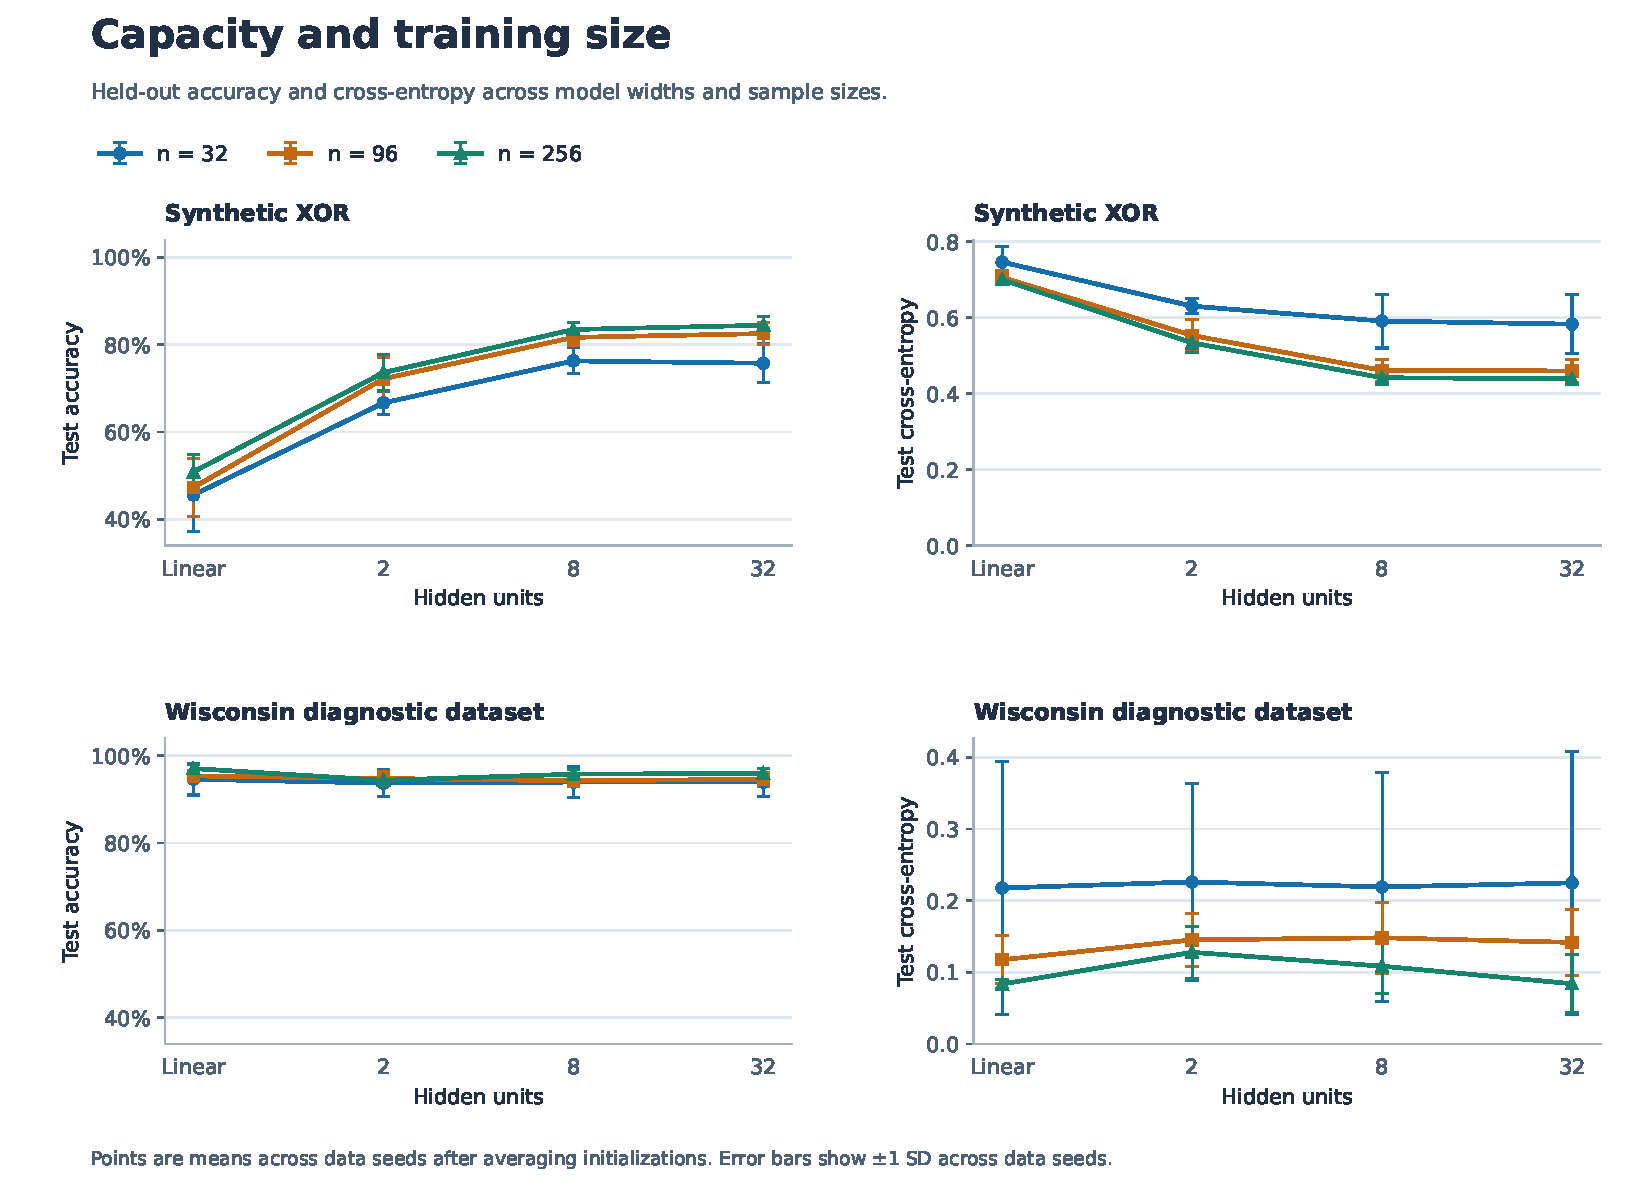
\includegraphics[width=\textwidth]{capacity.pdf}
\caption{Test accuracy and cross-entropy by sample size and hidden width.}
\end{figure}

\begin{table}[ht]
\centering
\small
\begin{tabular}{@{}lrccc@{}}
\toprule
Dataset & Training size & Logistic test acc.\ / loss & Width 8 & Width 32 \\
\midrule
Noisy XOR & 32 & 45.6\% / 0.747 & 76.3\% / 0.591 & 75.8\% / 0.583 \\
Noisy XOR & 96 & 47.3\% / 0.706 & 81.7\% / 0.462 & 82.6\% / 0.460 \\
Noisy XOR & 256 & 50.9\% / 0.700 & 83.5\% / 0.442 & 84.5\% / 0.440 \\
WDBC & 32 & 94.6\% / 0.218 & 94.0\% / 0.219 & 94.0\% / 0.225 \\
WDBC & 96 & 95.4\% / 0.118 & 94.3\% / 0.148 & 94.6\% / 0.142 \\
WDBC & 256 & 97.1\% / 0.084 & 95.8\% / 0.109 & 96.0\% / 0.084 \\
\bottomrule
\end{tabular}
\caption{Mean test accuracy / cross-entropy over 15 runs.}
\end{table}

On XOR at $n=256$, going from 2 to 8 hidden units raised accuracy from 73.6\% to 83.5\%, and going from 8 to 32 added about one more percentage point. At width 32, growing the training set from 32 to 256 examples raised mean accuracy by 8.7 percentage points and cut mean cross-entropy by 0.144. At $n=32$, width 32 has lower cross-entropy than width 8 but slightly lower accuracy, because cross-entropy also scores the probabilities the model assigns. On WDBC the linear baseline already separates most held-out cases, and extra width under this unregularized protocol brings no consistent test gain.

\section{Regularization}

\begin{figure}[ht]
\centering
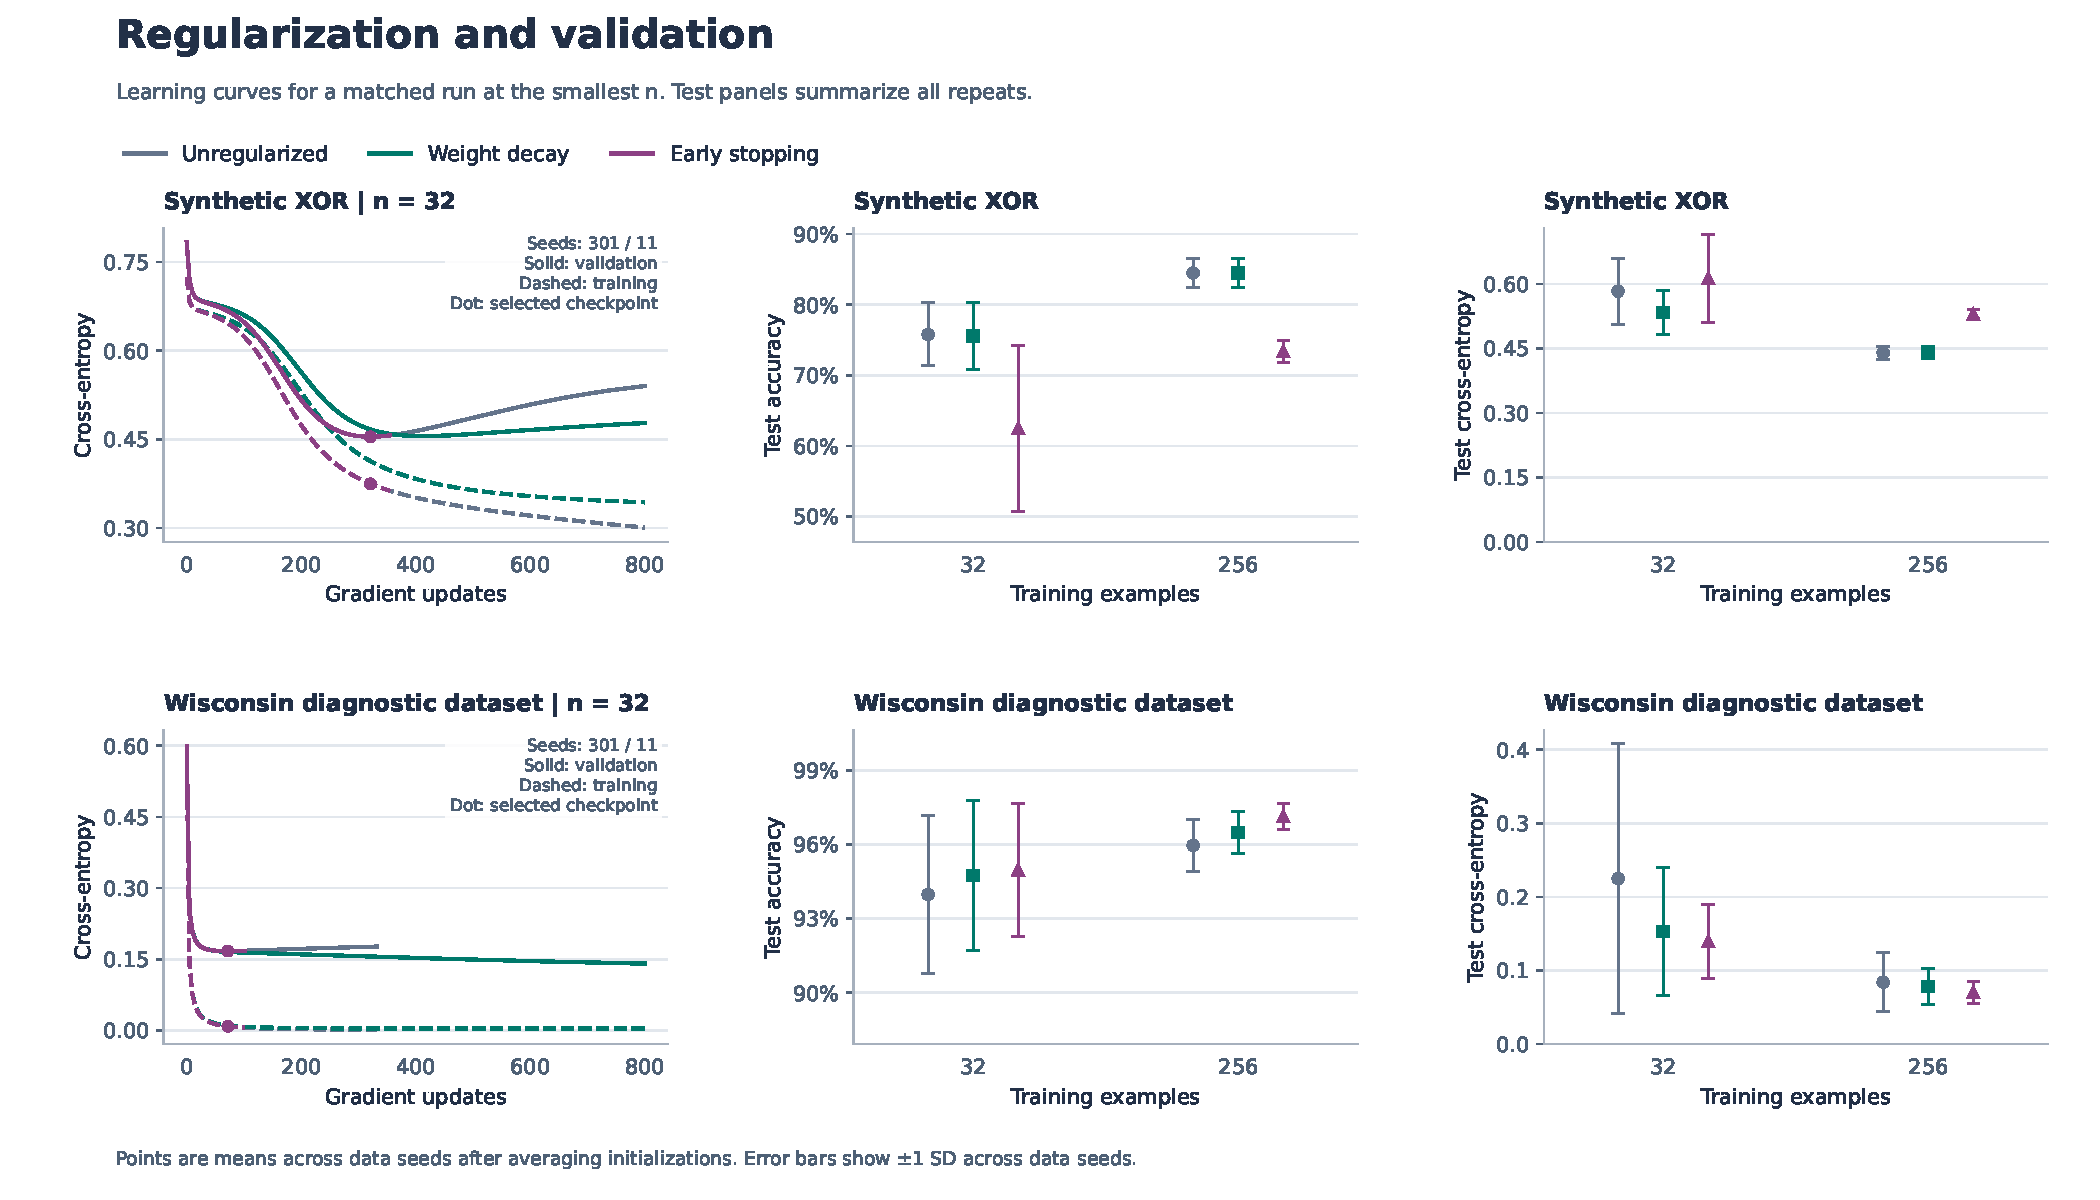
\includegraphics[width=\textwidth]{regularization.pdf}
\caption{Regularization test loss and matched training and validation curves.}
\end{figure}

\begin{table}[ht]
\centering
\small
\begin{tabular}{@{}lrccc@{}}
\toprule
Dataset & Training size & Unregularized & Weight decay & Early stopping \\
\midrule
Noisy XOR & 32 & 75.8\% / 0.583 & 75.6\% / 0.534 & 62.5\% / 0.613 \\
Noisy XOR & 256 & 84.5\% / 0.440 & 84.5\% / 0.440 & 73.3\% / 0.529 \\
WDBC & 32 & 94.0\% / 0.225 & 94.7\% / 0.153 & 95.0\% / 0.139 \\
WDBC & 256 & 96.0\% / 0.084 & 96.5\% / 0.078 & 97.1\% / 0.070 \\
\bottomrule
\end{tabular}
\caption{Mean test accuracy / cross-entropy for the width-32 network over the same 15 seed pairs.}
\end{table}

All 60 weight-decay runs picked the penalty with the lowest terminal validation cross-entropy in the tuning grid (\texttt{results/tuning.csv}). Early stopping checked validation loss after every update, including those between plotted points. Each run used the test set only after its model was selected.

On noisy XOR with 32 training examples, all 15 weight-decay runs selected $\lambda=0.005$, and weight decay lowered test cross-entropy in 14 of 15 matched runs. Averaging the three paired differences within each data seed gives a mean change of $-0.049$ (sample SD 0.041 across five seeds). Mean accuracy fell by only 0.2 percentage points, since cross-entropy also reflects the probability assigned to the observed class. At 256 examples, loss fell in 8 of 15 pairs and both methods averaged 0.440 to three decimals.

Early stopping on XOR selected update 144 on average at 32 examples, but the checkpoints fell into two groups. Eight of 15 runs restored updates 0 to 7, and the other seven restored updates 242 to 354. At 256 examples, five runs restored updates 4 to 9 and the other ten restored updates 460 to 800. Every run that restored a checkpoint near initialization lost test accuracy against its matched unregularized fit. In those runs the validation plateau triggered patience before the network had learned the XOR boundary.

On WDBC with 32 examples, early stopping reduced mean test loss from 0.225 to 0.139 while mean accuracy rose from 94.0\% to 95.0\%. Weight decay chose the three penalties (0.0005, 0.005, 0.05) in 6, 2 and 7 runs at 32 examples, and in 7, 8 and 0 runs at 256 examples. The run table (\texttt{results/runs.csv}) records the selected checkpoints and penalties for each seed pair.

\section{Random-label control}

\begin{figure}[ht]
\centering
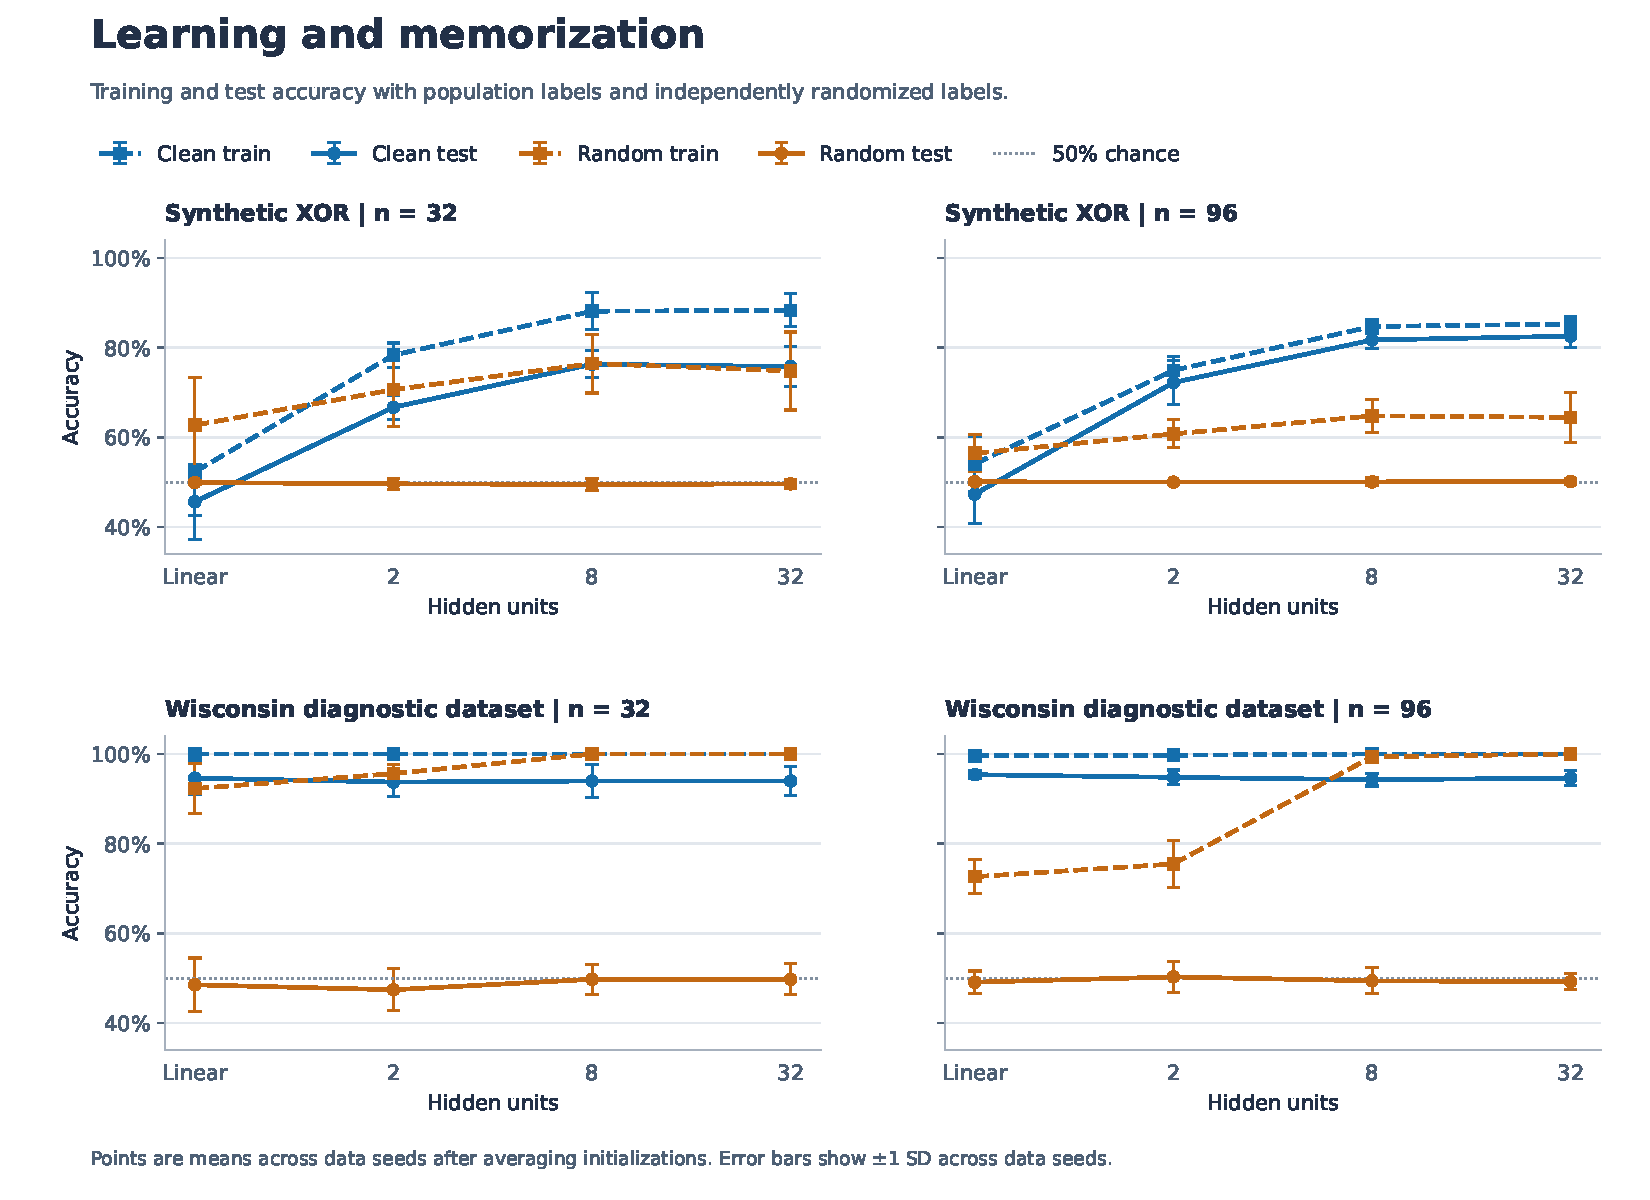
\includegraphics[width=\textwidth]{random_labels.pdf}
\caption{Train and held-out accuracy when labels are independently randomized.}
\end{figure}

The random controls keep the same features, sample membership and initial weights. Training, validation and test labels are drawn independently from $\Bernoulli(0.5)$ using separate streams, and each data seed fixes one draw per split for all paired model comparisons. A model cannot use features to predict independent test labels, so expected test accuracy is 50\%. Fitting random labels in this way follows the memorization test of Zhang et al.\ \cite{zhang2017}.

\begin{table}[ht]
\centering
\small
\begin{tabular}{@{}lrccc@{}}
\toprule
Dataset & Training size & Width-32 train accuracy & Test accuracy & Test loss \\
\midrule
Noisy XOR & 32 & 74.8\% & 49.6\% & 1.009 \\
Noisy XOR & 96 & 64.4\% & 50.2\% & 0.741 \\
WDBC & 32 & 100.0\% & 49.8\% & 2.470 \\
WDBC & 96 & 100.0\% & 49.2\% & 1.661 \\
\bottomrule
\end{tabular}
\caption{Width-32 results under random labels.}
\end{table}

The real-data features allowed complete memorization at these sizes under the width-32 training regime. At $n=32$, logistic regression on the same randomized WDBC data fit 92.3\% of the assignments, which is plausible with 30 input features and a bias. The width-32 test loss of 2.470 is far above the $\log 2\approx0.693$ of always predicting 0.5, because the model assigns confident probabilities to outcomes that are independent of the inputs. On the two-dimensional synthetic features, the same width and optimizer only partly fit random labels within the cap. The control measures the fit reached under each protocol, so it cannot establish how many arbitrary labels any architecture could fit.

The random-label audit (\texttt{RANDOM\_LABELS.md}) confirms that the drawn labels are independent of the features and across splits. Under this construction each run's test accuracy follows an exact $\operatorname{Binomial}(n_{\text{test}},0.5)$ null, and 229 of the 240 random-label runs fall inside its central 95\% interval.

\section{Compute budgets and controlled diagnoses}

\begin{figure}[ht]
\centering
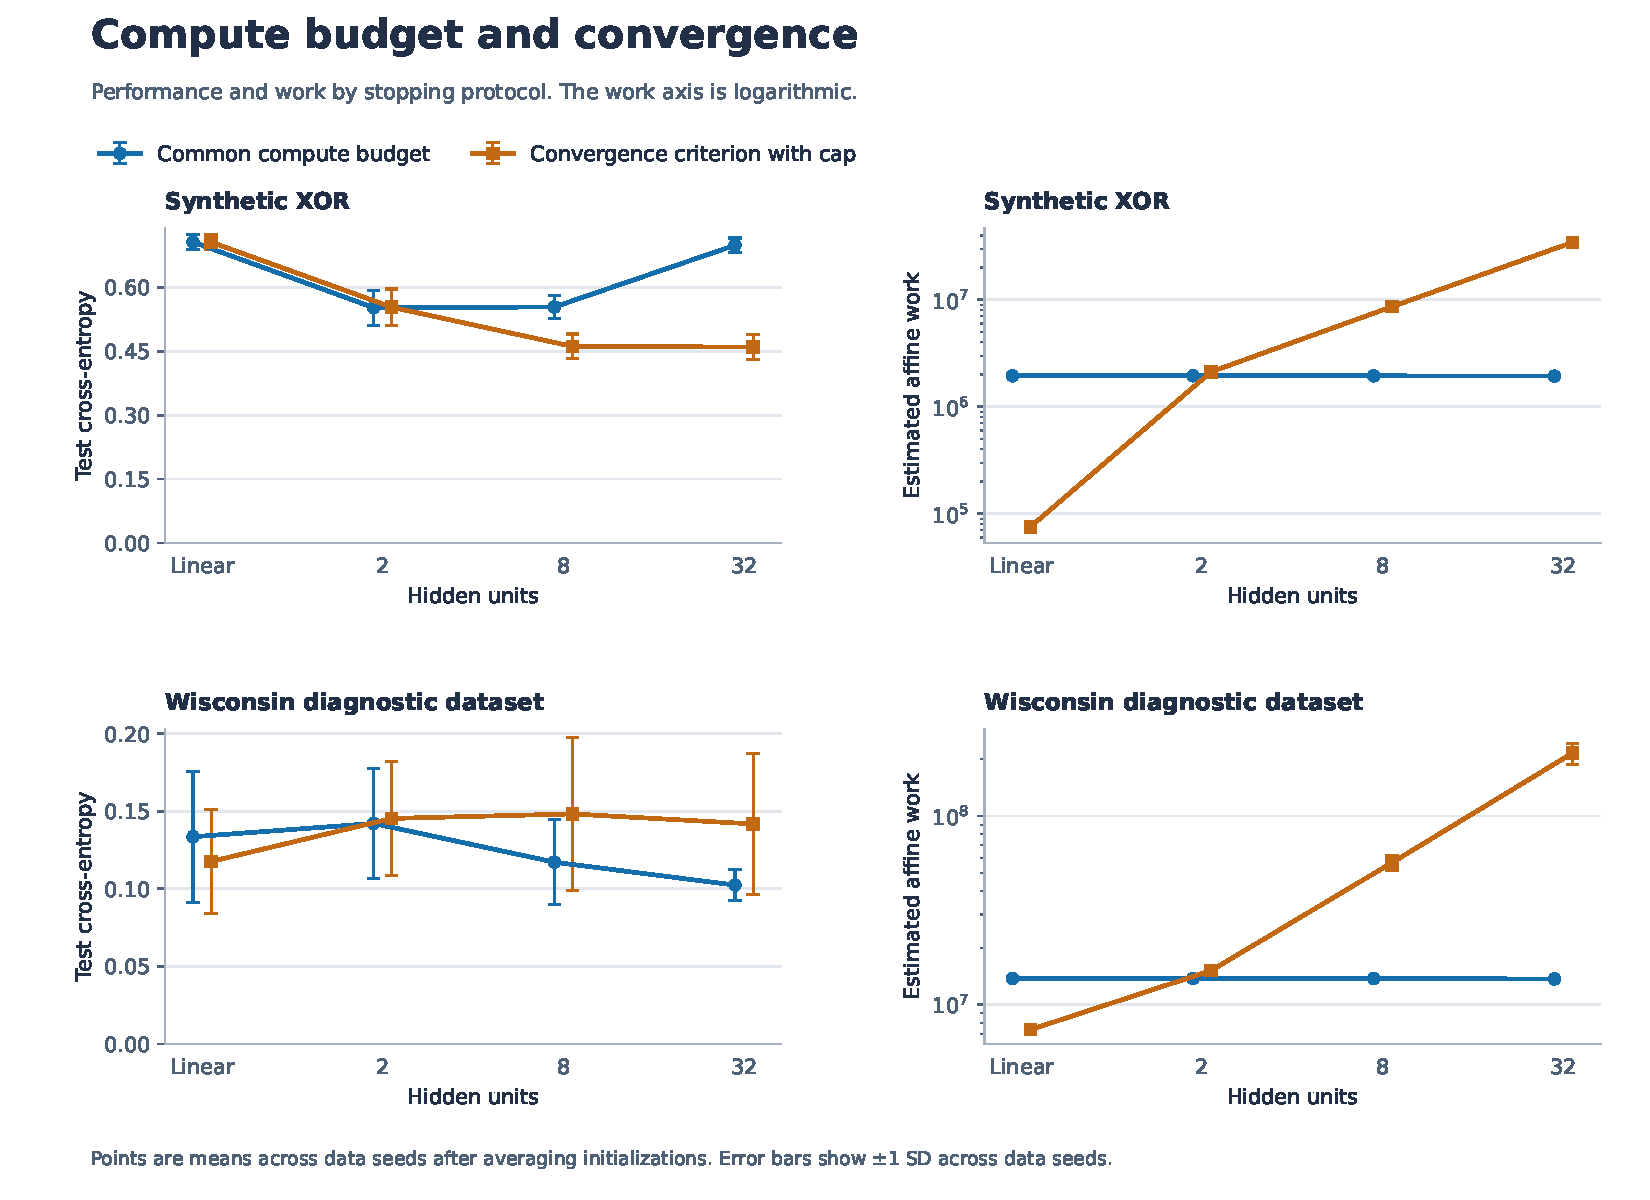
\includegraphics[width=\textwidth]{budget.pdf}
\caption{Test loss and estimated affine work under both budget rules.}
\end{figure}

At $n=96$ on each dataset, one checkpoint is a full training forward and gradient pass plus one validation forward pass. Its affine multiply-accumulate count is $(2n+n_v)d$ for logistic regression and $(2n+n_v)m(d+1)$ for the network, where $n_v$ is the validation size. The count covers the matrix and vector products for both affine layers and their weight gradients. Biases, elementwise operations, logging, final scoring and data preparation are left out. It is an architecture-sensitive compute proxy and does not measure elapsed time.

The common ceiling is 181 checkpoints of width 8 on the same dataset, which is 1,946,112 affine terms on XOR and 13,735,728 on WDBC. Each model gets the largest whole number of updates whose checkpoints fit, counting both the initial and the terminal checkpoint. Width 32 therefore receives 44 updates, width 8 receives 180 and width 2 receives 723. Logistic regression costs much less per update, so the same ceiling gives it 2,171 updates on XOR and 1,495 on WDBC, more than the 800-update cap of the other rule. That other regime stops on the gradient norm or after 800 updates, as defined above.

Despite its name, the second rule seldom reaches convergence for the networks. On XOR, widths 8 and 32 stopped at the cap in all 15 runs, with mean terminal gradient norms of 0.016 and 0.017 against the 0.005 threshold. Width 2 stopped at the cap in 13 of 15 runs and converged in the other 2. Logistic regression converged in all 15 runs after 83 updates on average, and no other width converged on XOR. On WDBC, 6 of 15 runs at widths 8 and 32 and 13 of 15 at width 2 reached the cap, as did all 15 logistic runs. For the networks on XOR this regime works as a fixed 800-update budget. Its compute is 1.1 times the common ceiling at width 2, 4.4 times at width 8 and 17.7 times at width 32. On WDBC the ratios are 1.1, 4.1 and 15.7, and logistic regression uses 0.54 times the ceiling.

\begin{table}[ht]
\centering
\small
\begin{tabular}{@{}ll>{\centering\arraybackslash}p{4.4cm}>{\centering\arraybackslash}p{4.4cm}@{}}
\toprule
Dataset & Width & Fixed budget: updates, test acc.\ / loss & Gradient rule with cap: updates, test acc.\ / loss \\
\midrule
Noisy XOR & Logistic & 2,171, 47.3\% / 0.707 & 83, 47.3\% / 0.706 \\
Noisy XOR & 2 & 723, 72.2\% / 0.553 & 788, 72.2\% / 0.554 \\
Noisy XOR & 8 & 180, 74.6\% / 0.554 & 800, 81.7\% / 0.462 \\
Noisy XOR & 32 & 44, 49.4\% / 0.699 & 800, 82.6\% / 0.460 \\
WDBC & Logistic & 1,495, 94.7\% / 0.134 & 800, 95.4\% / 0.118 \\
WDBC & 2 & 723, 94.9\% / 0.142 & 797, 94.8\% / 0.145 \\
WDBC & 8 & 180, 95.4\% / 0.117 & 743, 94.3\% / 0.148 \\
WDBC & 32 & 44, 96.4\% / 0.102 & 710, 94.6\% / 0.142 \\
\bottomrule
\end{tabular}
\caption{Both budget rules at $n=96$. Update counts under the gradient rule are means over 15 runs.}
\end{table}

The budget affects the two datasets differently. On XOR at equal compute, width 32 is the worst network, since 44 updates leave it near its initial loss of about 0.7. Width 8 gets 180 updates and reaches 74.6\%. A wider network needs more updates here, so its higher cost per update cancels any gain in capacity. Under the longer rule, width 32 reaches 82.6\%, about one point above width 8. On WDBC the fixed budget gives width 32 its best result, 96.4\% accuracy and 0.102 test loss. Its training loss is 0.069 there against 0.004 under the longer rule, and its test loss is lower. Stopping early is probably acting as implicit regularization, and the regularization section shows the same effect with explicit validation-based stopping. The WDBC gaps are about two points of accuracy, or about two of the 114 test cases, so they are suggestive and not firm. Extra training lowers training loss on both datasets but raised held-out loss only on WDBC.

\begin{figure}[ht]
\centering
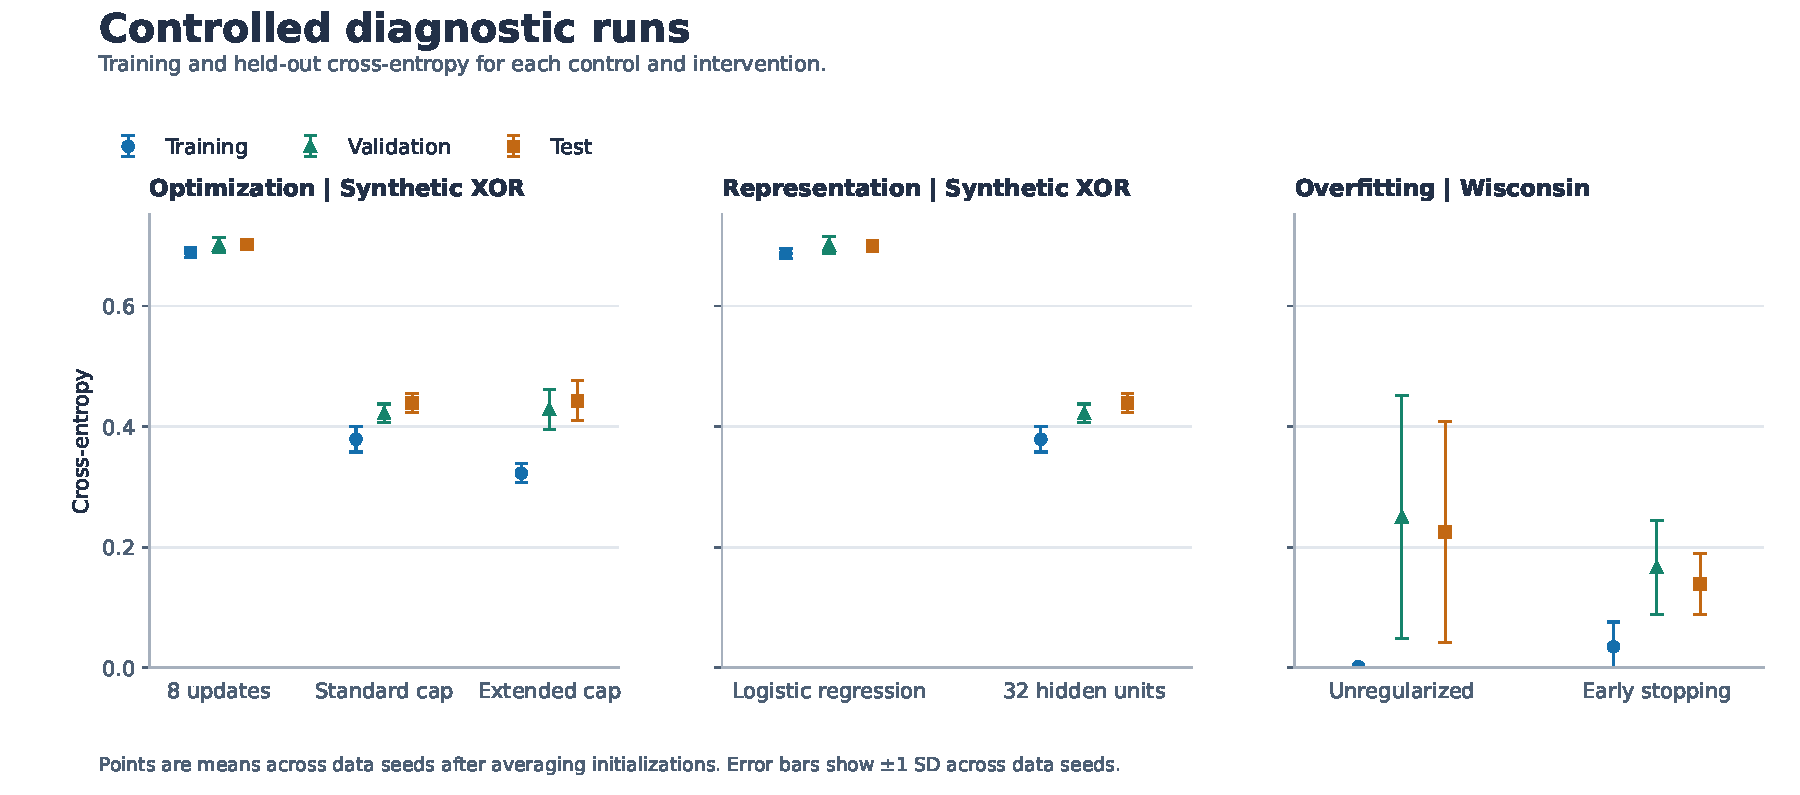
\includegraphics[width=\textwidth]{diagnostic.pdf}
\caption{Three matched changes for optimization, representation and overfitting.}
\end{figure}

\begin{table}[ht]
\centering
\small
\begin{tabular}{@{}>{\raggedright\arraybackslash}p{2.8cm}>{\raggedright\arraybackslash}p{4.3cm}ccc@{}}
\toprule
Diagnosis & Controlled change & Train loss & Validation loss & Test loss \\
\midrule
Optimization, XOR with $n=256$ & Same width 32, seed, learning rate and data. Increase allowance from 8 to 800 updates. & $0.689\to0.379$ & $0.701\to0.422$ & $0.702\to0.440$ \\
Optimization, continued & Same runs, 800 to 3,000 updates under the same gradient rule. & $0.379\to0.323$ & $0.422\to0.429$ & $0.440\to0.443$ \\
Representation, XOR with $n=256$ & Replace the linear model with width 32 and use the same gradient rule and 800-update cap. & $0.687\to0.379$ & $0.701\to0.422$ & $0.700\to0.440$ \\
Overfitting, WDBC with $n=32$ & Same width 32 and starting weights. Use the validation-selected checkpoint. & $0.002\to0.035$ & $0.250\to0.166$ & $0.225\to0.139$ \\
\bottomrule
\end{tabular}
\caption{Mean losses before and after each controlled change.}
\end{table}

\subsection{Optimization}

Width 32 trained for 8 updates sits at the initial loss of about 0.7, and 800 updates lower test loss to 0.440 with the same model, data and seed. The budget comparison above shows the same effect at 44 updates (49.4\% accuracy) against 800 (82.6\%). The 8-update run is a deliberately short control, so together these contrasts show that too few updates hurt a model that can fit this task. The 800-update fit still has a mean terminal gradient norm of 0.0168, so we trained the same runs for 3,000 updates. Training loss kept falling from 0.379 to 0.323, but test loss stayed at 0.443 (0.440 at 800) and test accuracy at 84.4\% (84.5\%). Only one of the 15 runs met the gradient threshold. Past 800 updates, further optimization lowers the training objective without improving held-out performance on this protocol, and validation loss rises slightly.

\subsection{Representation}

All 15 logistic fits meet the gradient threshold after 82 updates on average, so the linear model has converged. The width-32 network has not, since all 15 of its fits stop at the cap. These runs are the same as the 800-update runs in the first row of the table, with the same data and seeds. The population logistic objective is convex, and on this task its gradient is zero at zero weights and bias: both feature-label covariances vanish by symmetry and the labels are balanced. The population optimum is therefore the constant prediction of 0.5, with loss $\log 2\approx0.693$. The converged linear test loss of 0.700 matches this up to sampling noise, and the nonlinear network lowers it to 0.440. Because the linear fits converged, the evidence points to the linear model class as the limit and rules out optimization as the cause. The width-32 fits are still unconverged, so the comparison shows only that a nonlinear model fits much better.

\subsection{Overfitting}

In the WDBC comparison, validation-selected stopping lowers test cross-entropy from 0.225 to 0.139 while training cross-entropy rises from 0.002 to 0.035. Validation loss also falls, from 0.250 to 0.166, but validation loss is the selection criterion, so that drop is expected by construction and only test loss counts as evidence. Test accuracy rises from 94.0\% to 95.0\%, about one case out of 114. The matched initialization and the gap between near-zero training loss and much higher held-out loss support overfitting as the diagnosis. The accuracy change alone is too small to carry that claim.

\section{Runtime benchmark and convergence sensitivity}

The benchmark compares measured runtime with the estimated work above, and the sensitivity study varies the update cap and the learning rate. To reproduce both from the repository root:
\begin{verbatim}
python -m topic9.benchmark --output results
python -m topic9.sensitivity --output results
python -m topic9.figures results
\end{verbatim}
Add \texttt{-{}-quick} to either command for a one-seed smoke test in a separate output directory. The convergence study is deterministic. Timings depend on the machine, and the numbers below come from the archived run (Windows 11, an AMD64 processor with 16 logical cores, Python 3.13.4, NumPy 2.5.2 \cite{numpy}, one BLAS thread). Raw timings are in \texttt{results/runtime.csv}, per-condition summaries and the machine description are in \texttt{results/runtime\_summary.csv} and \texttt{results/runtime.json}, and the convergence runs are in \texttt{results/convergence.csv}.

\subsection{Runtime against estimated work}

The benchmark repeats the 16 conditions of the compute comparison: both datasets at $n=96$, logistic regression and widths 2, 8 and 32, under the common-compute rule and the gradient rule with the 800-update cap. Each of the 15 matched runs (the same data and initialization seeds as before) is timed five times after one untimed pass, with conditions interleaved within each repeat. The timed region is the whole \texttt{train} call. It includes the validation score computed at every checkpoint and excludes data preparation. Garbage collection is paused during timing. Every run reproduced its update count and stop reason in each repeat. The median coefficient of variation across the five repeats is between 1\% and 3\% for every condition except logistic regression on XOR under the gradient rule, where runs are short (0.004\,s) and it is 6\%.

\begin{figure}[ht]
\centering
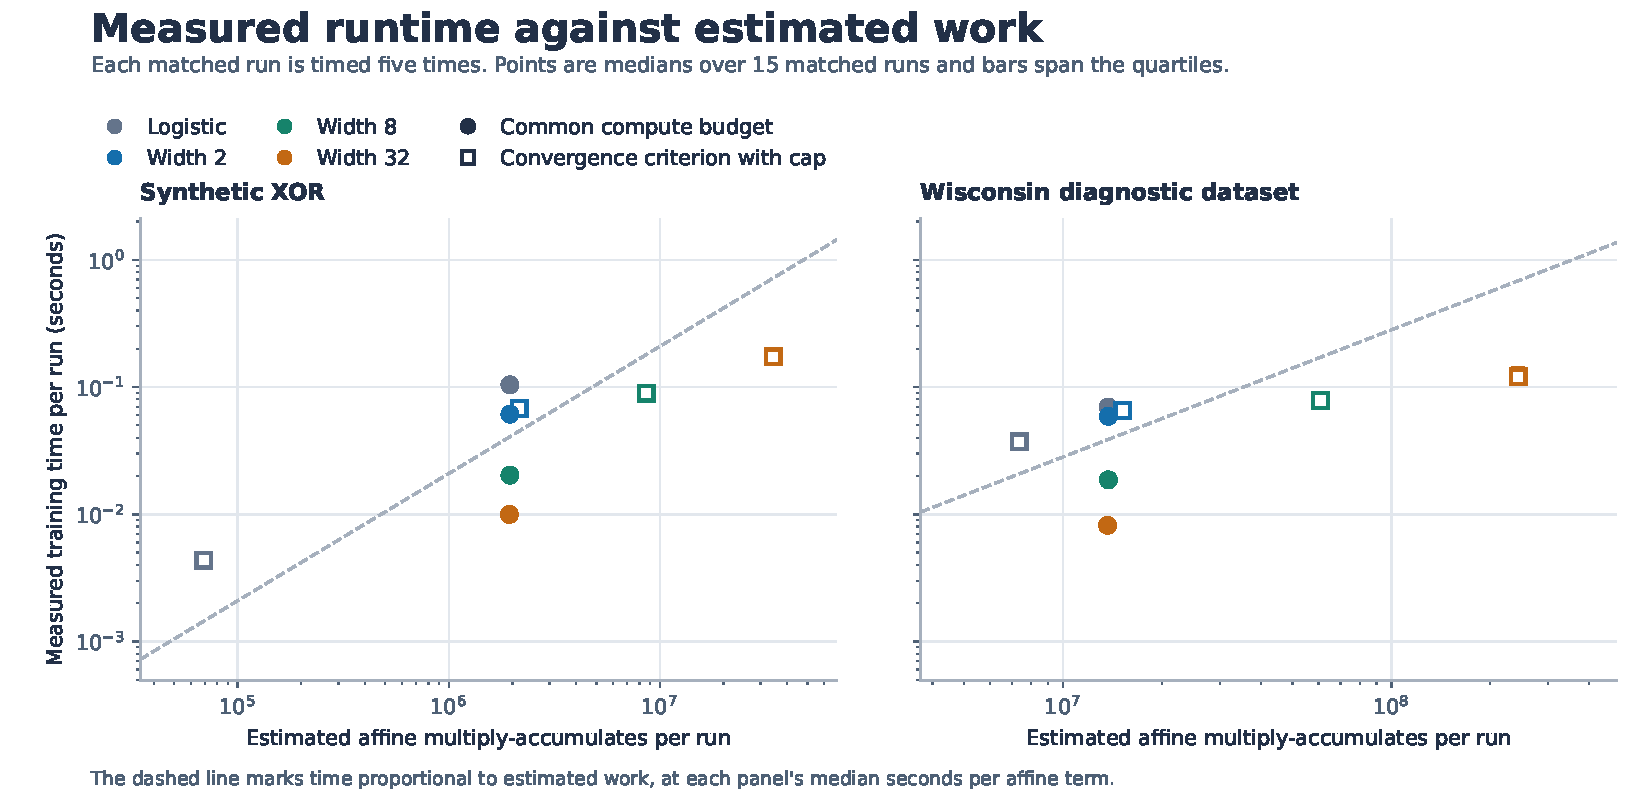
\includegraphics[width=\textwidth]{runtime.pdf}
\caption{Measured training time against estimated affine work.}
\end{figure}

\begin{table}[ht]
\centering
\small
\begin{tabular}{@{}ll>{\centering\arraybackslash}p{2.9cm}>{\centering\arraybackslash}p{3.1cm}>{\centering\arraybackslash}p{3.1cm}@{}}
\toprule
Dataset & Model & Common compute: updates, seconds & Gradient rule with cap: updates, seconds & $\mu$s per checkpoint (common / gradient) \\
\midrule
Noisy XOR & Logistic & 2,171, 0.104 & 83, 0.0044 & 48.0 / 51.7 \\
Noisy XOR & Width 2 & 723, 0.061 & 788, 0.068 & 84.5 / 86.0 \\
Noisy XOR & Width 8 & 180, 0.020 & 800, 0.090 & 111.9 / 111.8 \\
Noisy XOR & Width 32 & 44, 0.010 & 800, 0.173 & 221.2 / 215.7 \\
WDBC & Logistic & 1,495, 0.070 & 800, 0.037 & 46.5 / 46.4 \\
WDBC & Width 2 & 723, 0.059 & 797, 0.065 & 81.4 / 81.8 \\
WDBC & Width 8 & 180, 0.019 & 743, 0.079 & 103.0 / 105.5 \\
WDBC & Width 32 & 44, 0.008 & 710, 0.121 & 181.7 / 169.7 \\
\bottomrule
\end{tabular}
\caption{Measured runtime. Times are medians over the 15 matched runs, and updates are means. A checkpoint is one update plus its validation score.}
\end{table}

Within a single model, measured time follows estimated work closely. The time per checkpoint is within about 7\% between the two budget rules, and the ratio of runtimes between the rules is close to the ratio of estimated work. For width 32 on XOR, the gradient rule uses 17.8 times the estimated work of the common budget and takes 17.3 times as long.

Across models, estimated work is a poor guide to runtime. At the common budget, which equalizes estimated work to within 1\% on each dataset, measured time still ranges from 0.010\,s (width 32) to 0.104\,s (logistic regression) on XOR, a factor of 10.5. On WDBC it ranges from 0.008\,s to 0.070\,s, a factor of 8.5. Estimated work per checkpoint grows 48-fold from logistic regression to width 32 on XOR (896 to 43,008 terms) and 33-fold on WDBC, but measured time per checkpoint grows only about 4.6-fold and 3.9-fold. A least-squares fit across the 16 condition medians on log scales gives a slope of 0.35 with $R^2=0.36$ for time against work, so work alone explains little of the variation across models. The cost models in \texttt{results/runtime.json} agree: predicting time from work alone has a median relative error of 83\%, predicting it from the number of checkpoints alone gives 39\%, and combining a per-checkpoint cost with a per-work cost gives 27\%. The best fit has a per-checkpoint cost that depends only weakly on width. That is consistent with interpreter and elementwise overhead, and with matrix products running faster per multiply-accumulate at larger sizes, but we did not test either explanation. The affine count compares widths fairly in its own units, yet ``equal estimated compute'' does not mean equal elapsed time, and in wall-clock terms it favors the wider networks. These timings are specific to this NumPy implementation on one machine.

\subsection{Convergence sensitivity on noisy XOR}

The study uses the unregularized network on noisy XOR with 256 training examples, widths 8 and 32, the same gradient threshold of 0.005, and the same 5 data and 3 initialization seeds. The cap sweep varies the cap from 100 to 3,200 updates at learning rate 0.2. The learning-rate sweep varies the rate from 0.05 to 1.6 with the cap held at 800. The two sweeps share the baseline setting, and all 360 runs finished with finite losses.

\begin{figure}[ht]
\centering
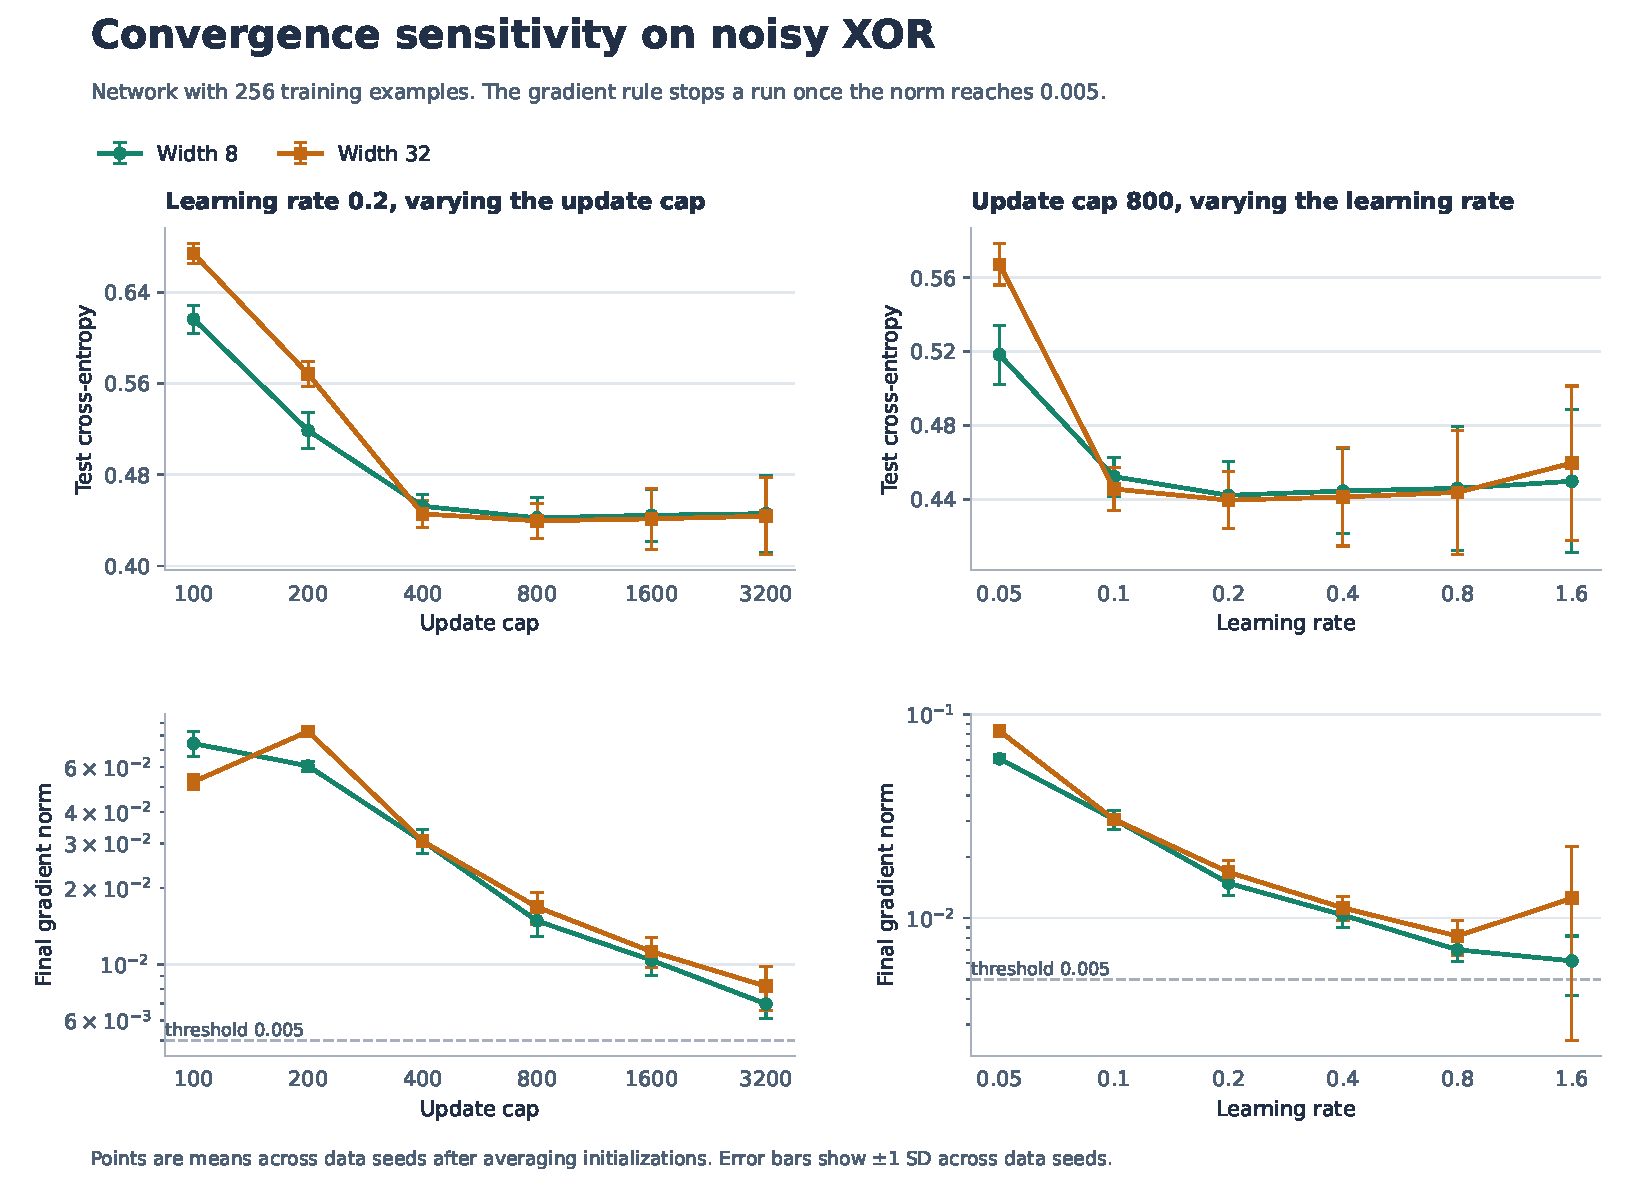
\includegraphics[width=\textwidth]{convergence.pdf}
\caption{Test loss and final gradient norm against update cap and learning rate.}
\end{figure}

\begin{table}[ht]
\centering
\small
\begin{tabular}{@{}llrrrrr@{}}
\toprule
Sweep & Setting & Converged & Mean updates & Train loss & Test loss & Final grad.\ norm \\
\midrule
Cap, rate 0.2 & cap 100 & 0 / 15 & 100 & 0.659 & 0.674 & 0.0526 \\
 & cap 200 & 0 / 15 & 200 & 0.550 & 0.568 & 0.0831 \\
 & cap 400 & 0 / 15 & 400 & 0.417 & 0.446 & 0.0306 \\
 & cap 800 & 0 / 15 & 800 & 0.379 & 0.440 & 0.0168 \\
 & cap 1,600 & 0 / 15 & 1,600 & 0.348 & 0.441 & 0.0112 \\
 & cap 3,200 & 1 / 15 & 3,152 & 0.320 & 0.444 & 0.0082 \\
\midrule
Rate, cap 800 & rate 0.05 & 0 / 15 & 800 & 0.548 & 0.567 & 0.0831 \\
 & rate 0.1 & 0 / 15 & 800 & 0.417 & 0.446 & 0.0306 \\
 & rate 0.4 & 0 / 15 & 800 & 0.348 & 0.441 & 0.0112 \\
 & rate 0.8 & 1 / 15 & 788 & 0.320 & 0.444 & 0.0082 \\
 & rate 1.6 & 4 / 15 & 734 & 0.291 & 0.460 & 0.0125 \\
\bottomrule
\end{tabular}
\caption{Width-32 convergence sensitivity. The baseline (rate 0.2, cap 800) appears once, under the cap sweep.}
\end{table}

Width 8 behaves the same way and is in \texttt{results/convergence.csv}. Its test loss is 0.442 at the baseline, and 9 of its 15 runs converge at rate 1.6.

The cap and the learning rate are largely interchangeable here. Settings with the same product of learning rate and cap give nearly the same results: rate 0.4 with cap 800 matches rate 0.2 with cap 1,600, and rate 0.1 with cap 800 matches rate 0.2 with cap 400. Across all 15 matched runs and both widths, the largest difference in either train or test loss is 0.0004. The pairs at a product of 40 (rate 0.05 against cap 200) and 640 (rate 0.8 against cap 3,200) differ by at most 0.0014. Until the step size gets large, the learning rate only rescales how many updates are needed.

Test loss and gradient norm point to different stopping times. Test loss reaches its minimum at a product of 160 (cap 800 at rate 0.2) and stays within 0.004 of it up to a product of 640. Training loss keeps falling, from 0.417 at cap 400 to 0.320 at cap 3,200, while test loss drifts up slightly after its cap-800 minimum of 0.440. The gradient norm falls more slowly still, from 0.0168 at cap 800 to 0.0082 at cap 3,200, so the 0.005 threshold is not reached within 3,200 updates at rate 0.2 for 14 of 15 runs at either width. The only runs that converge need a product of at least 640 (1 of 15 at width 8 and at width 32), and the rate-1.6 sweep reaches 9 of 15 at width 8 and 4 of 15 at width 32. The 800-update cap in the main experiments therefore sits on the held-out loss plateau but well short of the gradient criterion, so the cap decides the reported stopping reason there. At small caps, width 8 trains faster than width 32 (test loss 0.616 against 0.674 at cap 100), and the two are within 0.006 of each other from cap 400 onward.

The learning rate becomes unstable only at the top of the range. Training loss never increased from one update to the next in any run at rates up to 0.8, nor in any width-8 run at rate 1.6, but it did in 1 of the 15 width-32 runs at rate 1.6, with a largest increase of 0.004 between updates. Rate 1.6 also raises width-32 test loss to 0.460 and leaves the gradient norm higher than rate 0.8 (0.0125 against 0.0082), which suggests the step is starting to overshoot. We did not run larger rates. A learning rate of 0.2 with a cap of 800 gives the lowest mean test loss in both sweeps (0.440 at width 32 and 0.442 at width 8), but those runs should not be called converged.

\section{Limits and reproducibility}

The conclusions apply to these two datasets, the full-batch optimizer and learning rate used, the tested widths and sample sizes, and the fixed validation and test pools. The five data repetitions resample within a common reservoir, so repeating the outer split would capture another source of variation, especially for WDBC with 114 test cases. Values at the update cap describe performance under finite training. The compute comparison counts affine work only, and the runtime benchmark shows that this count does not predict elapsed time across model widths. The timings come from one machine. WDBC serves here as a benchmark for the coursework.

The repository \texttt{README.md} gives run commands. The run table (\texttt{results/runs.csv}), regularization curves (\texttt{results/curves.csv}), validation tuning grid (\texttt{results/tuning.csv}) and protocol metadata (\texttt{results/protocol.json}) keep the evidence behind the report. The archived run used Python 3.14.6, NumPy 2.5.2, scikit-learn 1.9.0, Matplotlib 3.11.1 \cite{matplotlib} and threadpoolctl 3.6.0 with one BLAS thread. The 3,000-update diagnostic was added later and run under Python 3.13.4 with the same package versions. A full rerun on that setup reproduced the update counts and stop reasons of all 1,350 archived rows. Losses matched except in two near-threshold random-label runs with width 2, which differed by up to 0.08, and one of those runs changed its test accuracy. We kept the archived rows and appended only the 15 new runs.

\begin{thebibliography}{10}

\bibitem{rumelhart1986}
D.~E. Rumelhart, G.~E. Hinton, and R.~J. Williams.
\newblock Learning representations by back-propagating errors.
\newblock \emph{Nature}, 323(6088):533--536, 1986.

\bibitem{glorot2010}
X.~Glorot and Y.~Bengio.
\newblock Understanding the difficulty of training deep feedforward neural networks.
\newblock In \emph{Proceedings of the 13th International Conference on Artificial Intelligence and Statistics (AISTATS)}, PMLR 9:249--256, 2010.

\bibitem{krogh1992}
A.~Krogh and J.~A. Hertz.
\newblock A simple weight decay can improve generalization.
\newblock In \emph{Advances in Neural Information Processing Systems 4}, pages 950--957, 1992.

\bibitem{prechelt1998}
L.~Prechelt.
\newblock Early stopping, but when?
\newblock In \emph{Neural Networks: Tricks of the Trade}, Lecture Notes in Computer Science 1524, pages 55--69. Springer, 1998.

\bibitem{zhang2017}
C.~Zhang, S.~Bengio, M.~Hardt, B.~Recht, and O.~Vinyals.
\newblock Understanding deep learning requires rethinking generalization.
\newblock In \emph{International Conference on Learning Representations (ICLR)}, 2017.

\bibitem{wdbc}
W.~Wolberg, O.~Mangasarian, N.~Street, and W.~Street.
\newblock Breast Cancer Wisconsin (Diagnostic).
\newblock UCI Machine Learning Repository, 1993.
\newblock \href{https://doi.org/10.24432/C5DW2B}{doi:10.24432/C5DW2B}.

\bibitem{sklearn}
F.~Pedregosa et~al.
\newblock Scikit-learn: Machine learning in Python.
\newblock \emph{Journal of Machine Learning Research}, 12:2825--2830, 2011.

\bibitem{numpy}
C.~R. Harris et~al.
\newblock Array programming with {NumPy}.
\newblock \emph{Nature}, 585:357--362, 2020.

\bibitem{matplotlib}
J.~D. Hunter.
\newblock Matplotlib: A 2D graphics environment.
\newblock \emph{Computing in Science \& Engineering}, 9(3):90--95, 2007.

\end{thebibliography}

\end{document}
